% Ch3.tex

\chapter[Math Equations]{Math Equations}
\label{cha:cha3}

This chapter shows you how to typeset math equations. We are not going to give a comprehensive description on this topic; but merely demonstrate this through some examples. 

Several sections of this chapter are directly taken from our paper \citep{TianPLA07}. We are not going to cite this paper everywhere in this chapter. However, keep in mind that the majority of the materials shown below come from this paper. 



%===========================
\section{Theoretical Background of Time Series Analysis}
\label{sec:theory}
%---------------
\subsection{R/S Analysis}

Denote the dynamics of the network traffic shown in Figure
\ref{fig:DelayS} as $x=\{x_k\}_{k=1}^N$, where $N$ is the length
of the sequence. This sequence can be treated as fractal records
in time. Hurst invented the $R/S$ analysis method to study such
sequences. Later, Mandelbrot and
Feder further developed this method in fractal
theory.

\begin{figure}[htb!]
\begin{center}
	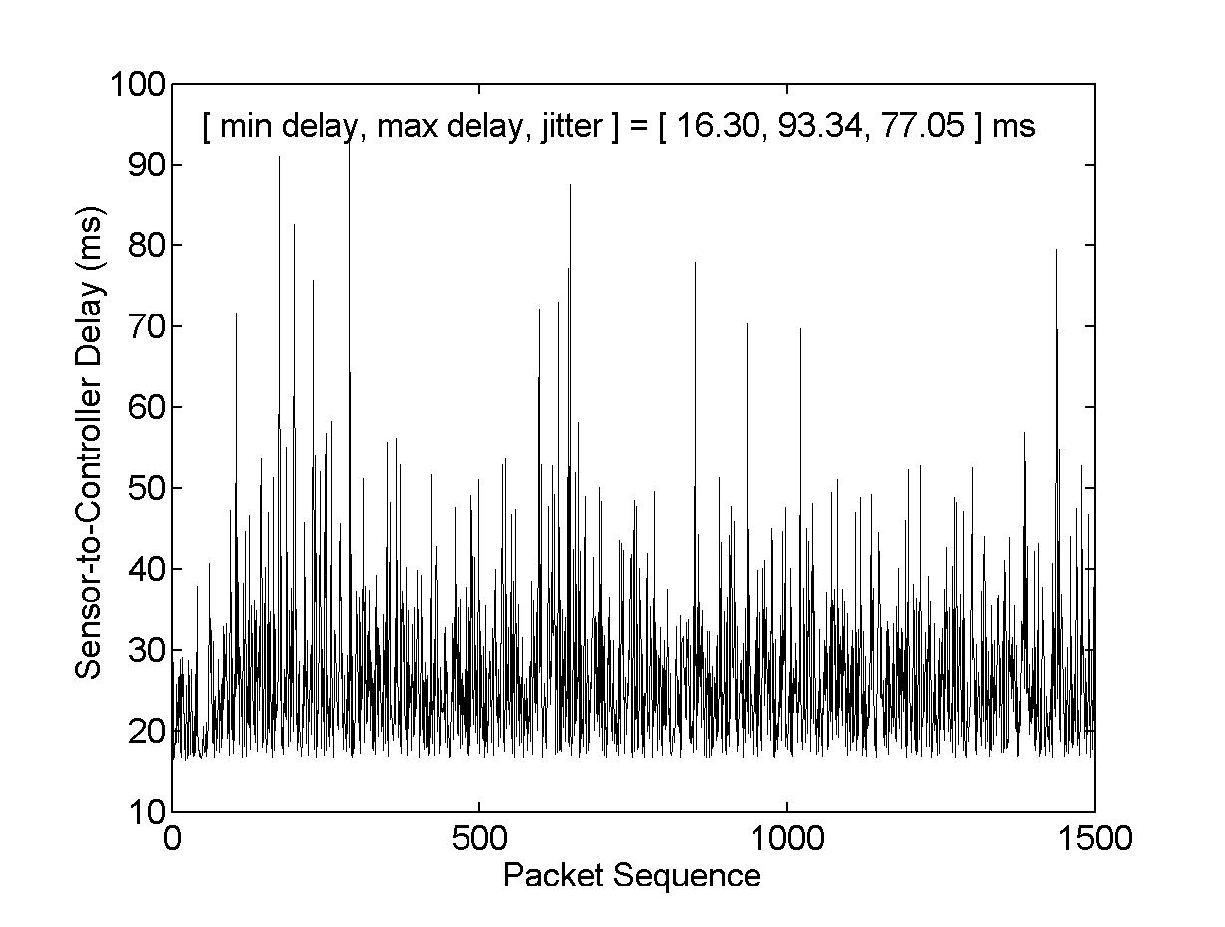
\includegraphics[scale=0.48]{./DelayS.eps}
%	\includegraphics[scale=0.39]{./Part3NCS/ComplexNet/images/DelayDist.eps}
\end{center}
	\caption[Sensor-to-controller delay]{Sensor-to-controller delay.}
	\label{fig:DelayS}
\end{figure}


For any fractal records in time $x=\{x_k\}_{k=1}^N$ and any $2\le n\le N$,
define
%
\begin{equation} <x>_{n}=\frac{1}{n}\sum_{i=1}^{n}x_i \end{equation}
%
\begin{equation} X(i,n)=\sum_{u=1}^i[x_u-<x>_{n}] \end{equation}
%
\begin{equation} R(n)=\max_{1\le i\le n}X(i,n)-\min_{1\le i\le n}X(i,n) \end{equation}
%
\begin{equation} S(n)=[\frac{1}{n}\sum_{i=1}^{n}(x_i-<x>_{n})^2]^{1/2} \end{equation}

Hurst found that
%
\begin{equation} R(n)/S(n) \ \sim\ (\frac{n}{2})^H \end{equation}
where $H$ is called the {\it Hurst exponent}.

As $n$ changes from $m$ to $N$, we obtain $N-m+1$ points
in $\ln(n)$ v.s. $\displaystyle{\ln(R(n) \over S(n))}$
 plane. Then, we can calculate the Hurst exponent for the time series
using the least-square linear fit.

The Hurst exponent is usually used as a measure of complexity.
The trajectory
of the record is a curve with a fractal dimension $D=2-H$. Hence
a smaller $H$ means a more complex system.
When applied to fractional Brownian motion, if $H > \displaystyle{1 \over 2}$,
the system is said to be {\em  persistent}, which means that if
for a given time period $t$ the motion is along one direction,
then in the time succeeding $t$ it is more likely that the motion
will follow the same direction. For a system with $H < \displaystyle{1 \over 2}$,
the opposite holds, that is, the system is 
{\em antipersistent}. But when $H=\displaystyle{1 \over 2}$
the system produces Brownian motion, which is random.